\documentclass{article}
\usepackage{graphicx}
\usepackage{hyperref}
\usepackage{float}

\hypersetup{
    colorlinks=true,
    linkcolor=blue,
    filecolor=magenta,      
    urlcolor=cyan,
    pdfpagemode=FullScreen,
}
\graphicspath{{./images/}}

\begin{document}

\title{Predicting song origin with Machine Learning and Spark}
\author{Oriol Agost Batalla, Ferran Aran Domingo}
\date{\today}
\maketitle
\begin{abstract}
    This project explores the use of machine learning and Spark to predict the country of origin for songs based on their features. Initially, we aimed to determine if it was possible to predict when a music group would break up based on song release features. However, due to insufficient data, we shifted our focus to predicting the country of origin. We utilized a dataset from HuggingFace containing song features and a dataset from MusicBrainz with artist information. After merging and preprocessing the data, we trained a classification model using XGBoost, achieving an accuracy of 70\%. We also employed SHAP values to explain the model's predictions. Finally, we deployed the model in a Streamlit app, making it accessible to the public. This report details the methodology, challenges, and results of our project.
\end{abstract}

\section{Introduction}
The globalization of music has made it increasingly common to encounter songs from diverse cultures and countries. Identifying the origin of a song can provide valuable insights into its cultural context and influence. In this project, we aim to predict the country of origin of a song based on its features using machine learning techniques and Apache Spark.

The initial hypothesis of our project was to predict when a music group might break up based on their song release features. However, this hypothesis was discarded due to the lack of sufficient data on music group breakups and the absence of release dates in the song features dataset. Consequently, we shifted our focus to predicting the country of origin of songs, leveraging data from the HuggingFace and MusicBrainz datasets.

This report provides a comprehensive overview of our approach, including data preprocessing and integration, model training and evaluation, the use of SHAP values for explainability, and the deployment of our model in a Streamlit app. Our findings demonstrate the potential of machine learning in the field of music analytics and offer a framework for future research and applications.

\section{Data sources}
Our project utilized two primary datasets, whose combination enabled us to gather comprehensive information about songs, their corresponding artists and their country of origin, providing the needed information for our predictive model.

\subsection{HuggingFace dataset}
The HuggingFace dataset, available at \href{https://huggingface.co/datasets/maharshipandya/spotify-tracks-dataset}{HuggingFace}, contains various features of songs, such as danceability, energy, and popularity. This dataset is well-structured in Parquet format and is publicly available, achieving a Tim Berners-Lee (TBL) score of 4 stars.

\subsection{MusicBrainz dataset}
The MusicBrainz dataset, accessible at \href{https://data.metabrainz.org/pub/musicbrainz/data/json-dumps/20240608-001001/}{MusicBrainz}, provides information about musical artists, including their country of origin. This dataset is available in JSON format, also publicly accessible, and has a TBL score of 3 stars.
\section{Data preprocessing and integration}

\subsection{Data cleaning and merging}
We began by loading and examining the HuggingFace and MusicBrainz datasets using Apache Spark. The data cleaning process involved removing any irrelevant or duplicate records and standardizing the format of the datasets to ensure consistency. 

The following Spark operations were utilized:
\begin{itemize}
    \item \textbf{Filtering}: We removed artists whose origin country or name where not known. Also, rows with duplicate information where dropped.
    \item \textbf{Joining}: The datasets were joined on the artist name to merge song features with the corresponding artist's country of origin. This was achieved using the \texttt{join} function in Spark. Both an \texttt{inner join} and a \texttt{left antijoin} where employed to have those songs whose origin country are known and also those that are not.
    \item \textbf{Resampling}: Given the imbalance in the dataset (e.g., over 15,000 songs from the US compared to countries with only a few songs, check \autoref{fig:imbalance} for more details), we decided to remove countries with 500 or fewer songs. We then resampled the remaining countries to have 500 songs each to create a balanced dataset, whose distribution can be seen at \autoref{fig:balanced}.
\end{itemize}

\begin{figure}[H]
    \centering
    \noindent
    \makebox[\textwidth]{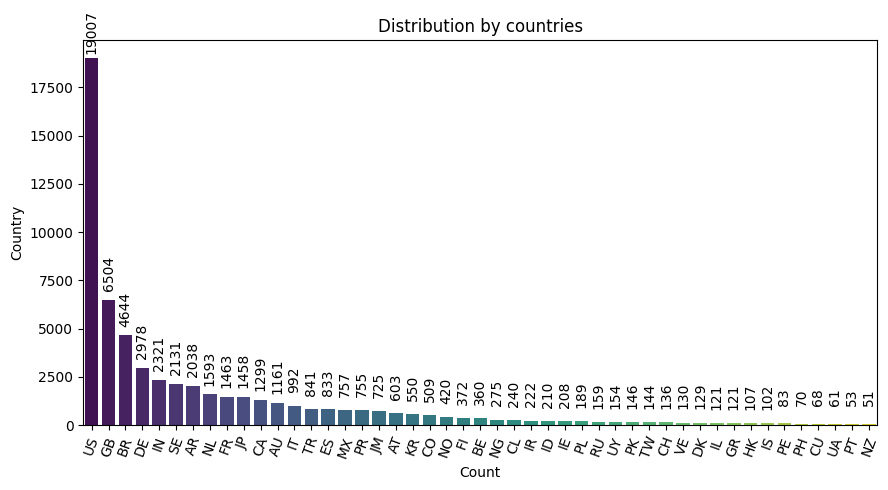
\includegraphics[scale=0.52]{images/songs-per-country.png}}
    \caption{Distribution of songs per country before resampling.}
    \label{fig:imbalance}
\end{figure}

\begin{figure}[H]
    \centering
    \noindent
    \makebox[\textwidth]{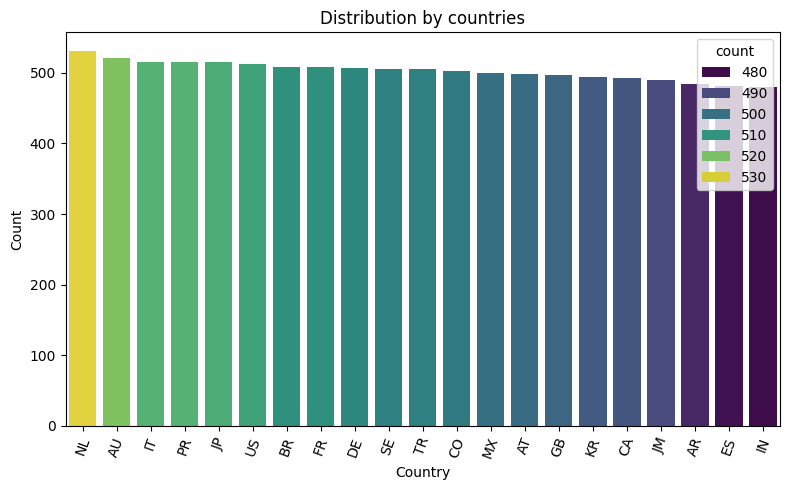
\includegraphics[scale=0.55]{images/balanced.png}}
    \caption{Distribution of songs per country after resampling.}
    \label{fig:balanced}
\end{figure}

\subsection{Handling imbalanced data}
The resampling process was crucial to ensure that our model did not become biased towards countries with a higher number of songs. By balancing the dataset, we aimed to provide a fair representation of each country's song features in the training process. The result is not perfectly balanced due to the way Spark implements \href{https://spark.apache.org/docs/latest/api/python/reference/pyspark.sql/api/pyspark.sql.DataFrame.sample.html}{its resampling methods}, prioritizing an efficient result over a perfectly balanced result, given that i doesn't matter that much to have the same exact number of samples per country.

\section{Modeling}

\subsection{Choice of models}
To explore the predictive capabilities of our dataset, we initially experimented with Spark's MLlib, specifically the RandomForest classifier. However, the accuracy was suboptimal at around 40\%. Seeking better performance, we turned to the XGBoost library, which is known for its efficiency and high performance in classification tasks.

\subsection{Training process}
The training process involved several key steps:
\begin{itemize}
    \item \textbf{Data Splitting}: We split the dataset into training and testing sets to evaluate our model's performance. As usual, an 80-20 split was used.
    \item \textbf{Feature Encoding}: Categorical features, such as musical genres and countries, were encoded using label encoders to convert them into a numerical format suitable for the model.
    \item \textbf{Model Training}: The XGBoost model was trained on the song features, with the country of origin as the target variable.
\end{itemize}

\subsection{Evaluation of models}
The performance of the models was evaluated using accuracy as the primary metric. The Spark MLlib RandomForest classifier achieved an accuracy of 40\%, whereas the XGBoost model significantly outperformed it with an accuracy of 70\%. Given the substantial improvement, we selected the XGBoost model for further analysis and deployment.\newline

One possible cause for the low accuracy of the RandomForest implementation of Spark MLlib is it not being able to handle more than 32 categories in a feature, which is a limitation that is not present on XGBoost. To overcome this limitation, we had to reduce the number of categories in the genre feature by grouping them into broader categories using Spark MLlib \texttt{QuantileDiscretizer}.

\section{Explainability}

\subsection{Use of SHAP values}
To understand the predictions made by our XGBoost model, we utilized \href{https://christophm.github.io/interpretable-ml-book/shap.html}{SHAP} (SHapley Additive exPlanations) values. SHAP values provide insights into the contribution of each feature to the model's predictions, enhancing the interpretability of the results.

\subsection{Visualizations}
We incorporated various visualizations to demonstrate the SHAP values:
\begin{itemize}
    \item \textbf{Force Plots}: These plots illustrate the contribution of each feature to a single prediction, showing how the presence or absence of certain characteristics pushes the prediction towards a particular country.
    \item \textbf{Summary Plots}: These plots provide an overview of feature importance across the entire dataset, highlighting the most influential features in predicting song origin for each country.
    \item \textbf{Decision Tree}: We also visualized the decision tree used by the XGBoost model to provide a clear understanding of the model's decision-making process, which can be seen in \autoref{fig:tree}, or full resolution image go \href{https://raw.githubusercontent.com/FerranAD/songmap/main/images/xgb_tree.png}{here}.
\end{itemize}

\begin{figure}[H]
    \centering
    \noindent
    \makebox[\textwidth]{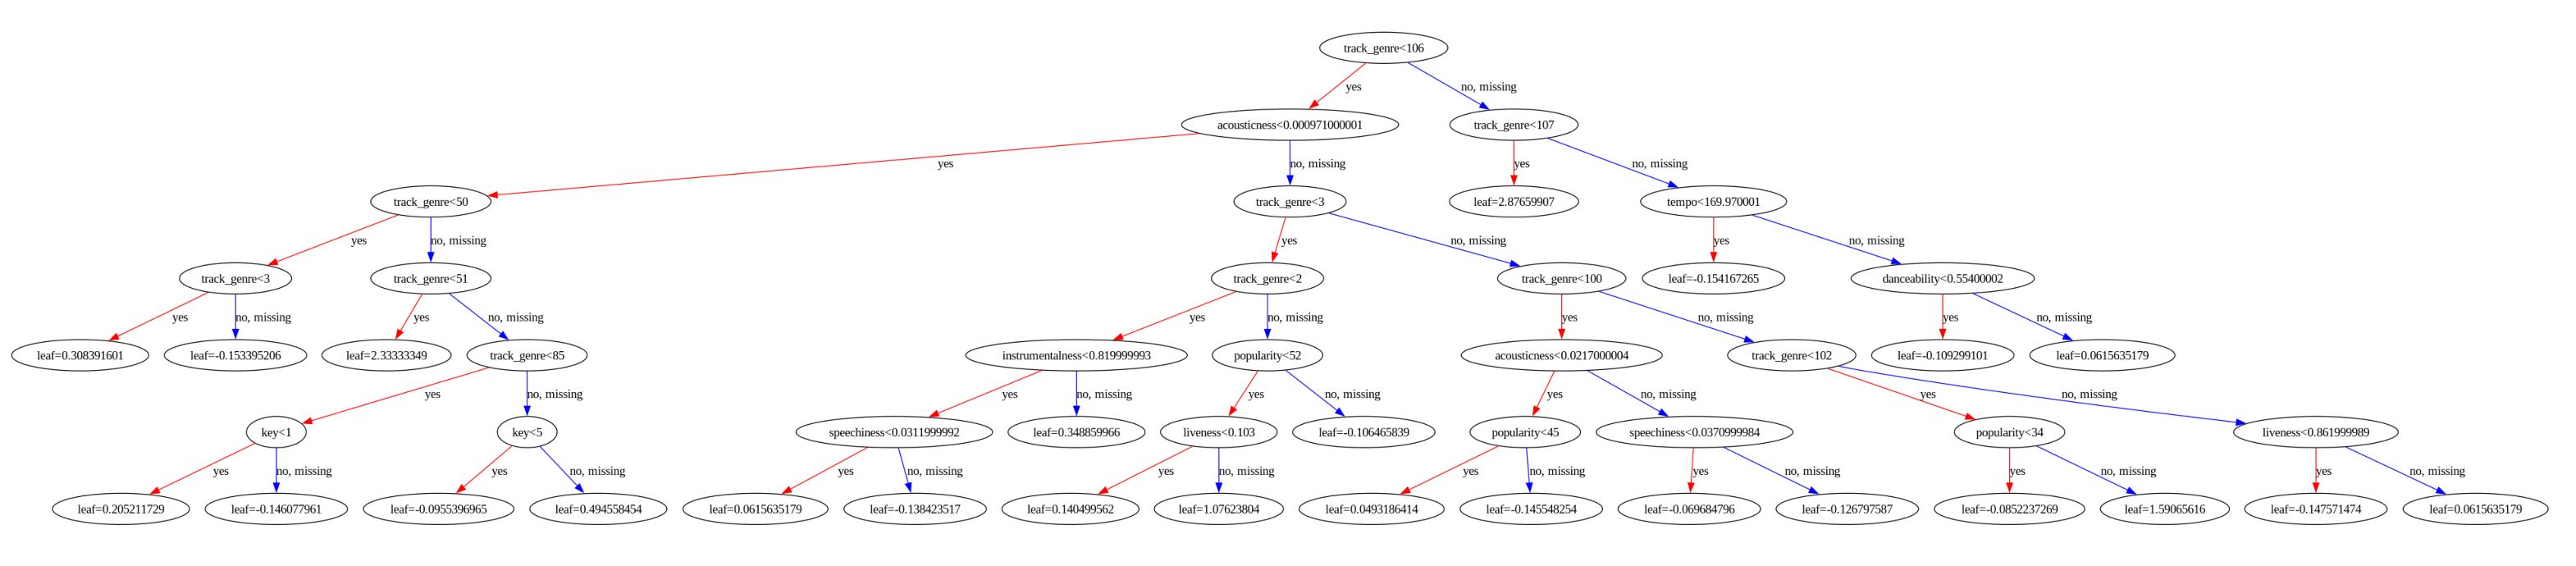
\includegraphics[scale=0.15]{images/tree.png}}
    \caption{XGBoost model decision tree.}
    \label{fig:tree}
\end{figure}

\subsection{Insights from model explainability}
By examining the SHAP values, we identified which features had the most significant impact on predicting the country of origin. This analysis revealed that features such as music genre, popularity, and speechiness were among the top contributors. The use of SHAP values allowed us to visualize the influence of these features through force plots and summary plots, offering a clear understanding of the model's decision-making process.\newline

For example, take the Netherlands summary plot at \autoref{fig:netherlands}, which is known to be the country of origin of many electronic music artists. The SHAP values for the Netherlands show that the model gives a lot of importance to the music genre feature, which is a good indicator that the model is learning patterns that are consistent with the cultural and musical characteristics of the country.\newline

\begin{figure}[H]
    \centering
    \noindent
    \makebox[\textwidth]{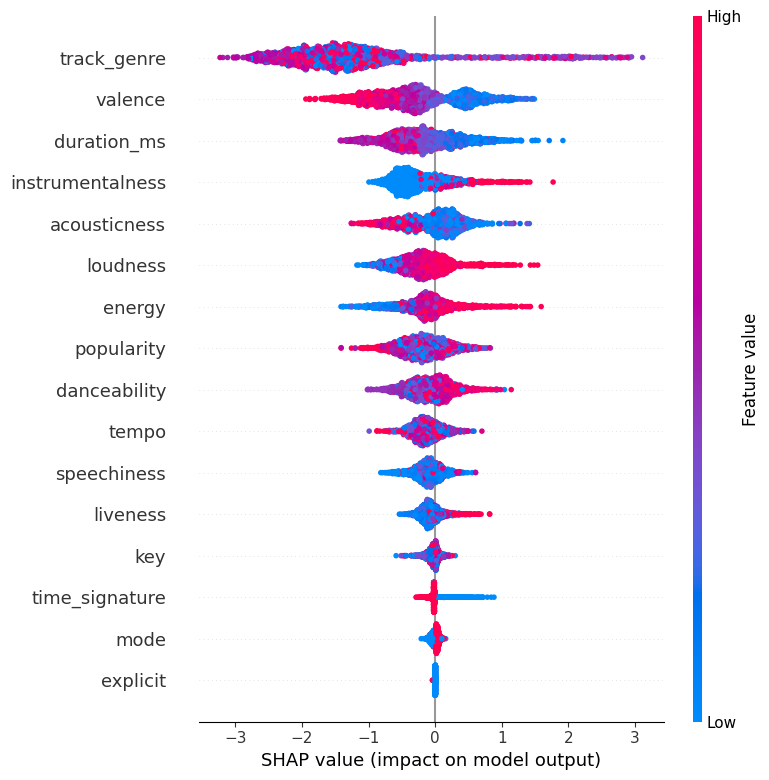
\includegraphics[scale=0.57]{images/netherlands.png}}
    \caption{Shap value summary plot for the Netherlands. The more distanced from zero the more important the feature is.}
    \label{fig:netherlands}
\end{figure}

On the other hand, we've got Canada at \autoref{fig:canada}, which is not as particularly known for any specific genre. The SHAP values for Canada show that the model gives importance to features like valence and popularity, which are more general characteristics that can be found in a wide variety of songs.

\begin{figure}[H]
    \centering
    \noindent
    \makebox[\textwidth]{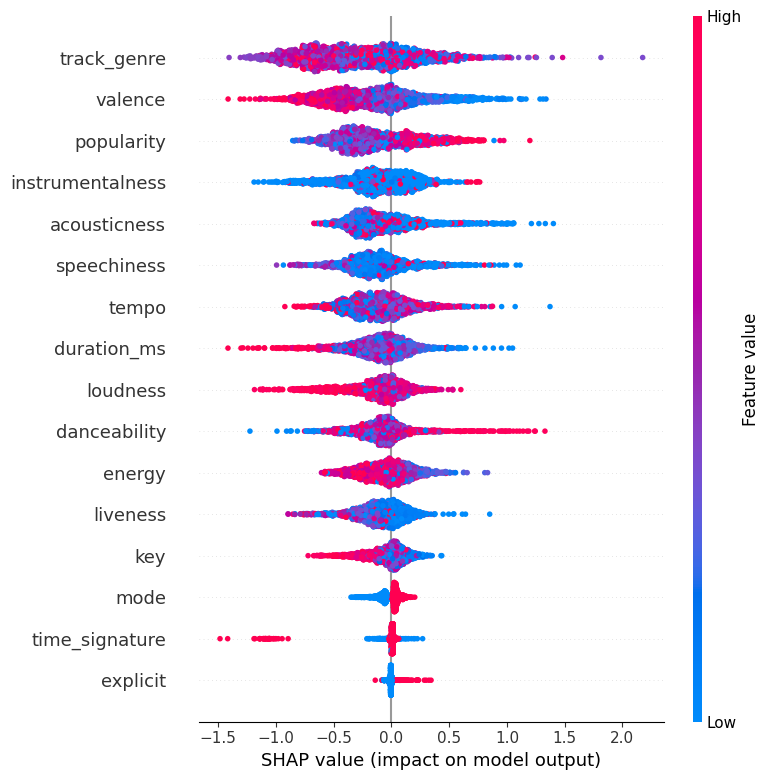
\includegraphics[scale=0.57]{images/canada.png}}
    \caption{Shap value summary plot for Canada.}
    \label{fig:canada}
\end{figure}

When looking at individual predictions, force plots help us understand why the model made a specific prediction. For example, in the force plot for a song (One Dance - Drake) predicted to be from Canada (and that actually is from a canadian artist), we can see that the danceability and popularity of the song contribute the most to the model's decision, as shown in \autoref{fig:force-plot-canada}.\newline

\begin{figure}[H]
    \centering
    \noindent
    \makebox[\textwidth]{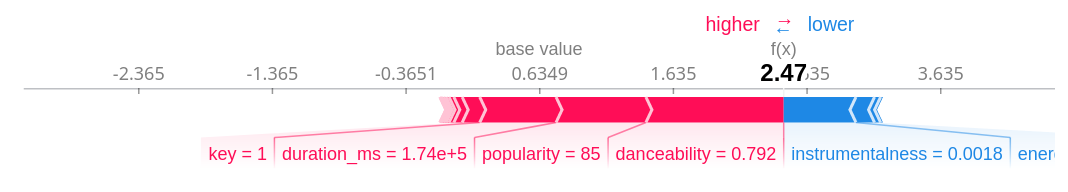
\includegraphics[scale=0.40]{images/force-plot-canada.png}}
    \caption{Force plot for canadian song. Red values push the prediction up, while blue values push it down.}
    \label{fig:force-plot-canada}
\end{figure}

If we take a look at an electronic music track (Rock Civilization - Technoboy's Undersound Mix - Headhunterz) predicted to be from the Netherlands, we can see that in this case the music genre takes te first place in the SHAP values, as shown in \autoref{fig:force-plot-netherlands}.\newline

\begin{figure}[H]
    \centering
    \noindent
    \makebox[\textwidth]{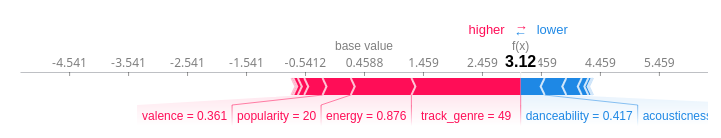
\includegraphics[scale=0.60]{images/force-plot-netherlands.png}}
    \caption{Force plot for netherlands song.}
    \label{fig:force-plot-netherlands}
\end{figure}

\section{Deployment}

\subsection{Streamlit app}
To make our model accessible to the public, we developed a Streamlit \href{https://songmap.xyz}{website}. Streamlit is a powerful tool for building interactive web applications with minimal code. The app allows users to input a song or artist name, which will then be searched on the dataset using Spark, and receive a prediction of the song's country of origin, along with the SHAP values explaining the model's decision.

\subsection{Dockerization and cloud deployment}
For ease of deployment, we containerized the Streamlit app using Docker. This approach ensures consistency across different environments and simplifies the deployment process. The Docker container was then deployed on Google Cloud Run.

The steps for local deployment can be found on the {Github repository}\href{https://github.com/FerranAD/songmap}, but it is as easy as:
\begin{enumerate}
    \item Clone the repository from GitHub.
    \item Build and run the Docker container using Docker Compose.
\end{enumerate}

\subsection{App content}
The Streamlit app features an intuitive user interface where users can search for songs and view predictions. The app also includes a "More Info" section that provides detailed explanations of the model's predictions using SHAP values, as well as visual representations of the decision tree used by the XGBoost model.

\section{Conclusion}
In this project, we successfully developed a machine learning model to predict the country of origin for songs based on their features, confirming that such features can tell enough of a song to infere its origin country. By leveraging Apache Spark for data preprocessing and XGBoost for model training, we achieved a high level of accuracy and gained valuable insights into the predictive power of various song attributes.

\section{Resources}

\begin{itemize}
    \item \href{https://github.com/FerranAD/songmap}{Github repository of this project, which contains the used notebooks, processed datasets, this report and the Streamlit app code.}
    \item \href{https://songmap.xyz}{Streamlit app website.}
    \item \href{https://raw.githubusercontent.com/FerranAD/songmap/main/images/xgb_tree.png}{Full resolution image of the XGBoost model decision tree.}
    \item \href{https://github.com/FerranAD/songmap/blob/main/preprocessing.ipynb}{Data preprocessing notebook.}
    \item \href{https://github.com/FerranAD/songmap/blob/main/analysis.ipynb}{Model training and analysis notebook.}
\end{itemize}

\end{document}